\documentclass[11pt,a4paper]{article}

% ---------------------------------------------------------------------------
% Objective 1 report: selecting a small language model for a retail kiosk
% Compile with:  pdflatex objective1_report.tex  (run twice for references)
% Figures are expected in ./figs/ (produced by make_figs.py).
% ---------------------------------------------------------------------------

\usepackage[margin=2.4cm]{geometry}
\usepackage[T1]{fontenc}
\usepackage{mathpazo}
\usepackage{microtype}
\usepackage{graphicx}
\usepackage{booktabs}
\usepackage{tabularx}
\usepackage{xltabular}
\usepackage{array}
\usepackage{multirow}
\usepackage{xcolor}
\usepackage{enumitem}
\usepackage{amsmath}
\usepackage{caption}
\usepackage{float}
\usepackage{tikz}
\usetikzlibrary{arrows.meta,positioning,shapes.geometric,fit}
\usepackage[hidelinks]{hyperref}

\definecolor{ink}{HTML}{0B0B0B}
\definecolor{ink2}{HTML}{52514E}
\definecolor{qblue}{HTML}{2A78D6}
\definecolor{qorange}{HTML}{EB6834}
\definecolor{qaqua}{HTML}{1BAF7A}
\definecolor{boxfill}{HTML}{F3F7FD}

\captionsetup{font=small,labelfont=bf}
\setlist{itemsep=2pt,topsep=4pt}
\renewcommand{\arraystretch}{1.18}
\newcolumntype{L}{>{\raggedright\arraybackslash}X}

% Placeholders: replace before submission
\newcommand{\placeholder}[1]{\textcolor{red}{[#1]}}
\newcommand{\reportauthor}{\placeholder{Author name}}
\newcommand{\reportaffil}{\placeholder{Institution / programme}}
\newcommand{\reportdate}{11 September 2026}

\title{\textbf{Selecting a Small Language Model for an Offline\\Retail Kiosk Assistant}\\[4pt]
\large Objective 1: Model Selection Report}
\author{\reportauthor\\\small\reportaffil}
\date{\reportdate}

\begin{document}
\maketitle

\begin{abstract}
\noindent
A retail kiosk assistant has to find products, answer questions from product data, hand customers over to staff, and
refuse what it cannot do, all on modest in-store hardware with no cloud connection. This report selects the language
model for such an assistant. Six open small language models (0.8--4\,billion parameters) were tested on a
fictional watch retailer, using six kiosk tools and a 370-case evaluation set with fixed expected answers. Testing ran in
four stages: screening, quantization, a head-to-head on a 292-case held-out test split, and speed and memory
measurement on CPU and on an integrated GPU. All decision rules were fixed before any results were seen. Every
comparison is paired and reported with 95\% confidence intervals.
\textbf{Qwen3.5-4B at 4-bit (Q4\_K\_M)} is selected for GPU-equipped kiosks: it passed 81\% of test cases, and was
significantly better than every other configuration. \textbf{Qwen3.5-2B at 8-bit (Q8\_0)} is selected for CPU-only
kiosks: it passed 74\% within 2.7\,GB of RAM.
Neither model reaches the 80\% tool-call accuracy cut-off that was set in advance (75\% and 74\%). A failure analysis
traces most misses to two behaviours, asking unnecessary questions and failing to call staff, both of which are
candidates for prompt and tool-design fixes in the next objective. A blind rubric evaluation of reply quality,
checked against human scores, confirms the ranking.
\end{abstract}

\tableofcontents
\vspace{6pt}
\hrule

% ===========================================================================
\section{Introduction}
% ===========================================================================

In-store kiosks are a natural place for a conversational assistant. A customer can ask for ``a formal watch for my
father around 15,000 rupees'' instead of browsing filters. A kiosk, however, imposes constraints that a cloud chatbot
does not:
\begin{itemize}
  \item it runs on a small, fanless PC or an entry-level laptop-class machine;
  \item it should keep working without a network connection;
  \item it must never invent a product, a price or a store policy;
  \item it must hand the customer to a human for anything it cannot do.
\end{itemize}

Published kiosk deployments of small models share a common architecture, and this project adopts it:
\begin{itemize}
  \item \textbf{the model talks}: a small language model handles the conversation;
  \item \textbf{tools act}: structured function calls search the catalogue, check stock, compare products and call staff;
  \item \textbf{retrieval knows}: product and policy text is supplied to the model rather than memorised;
  \item \textbf{a fallback refuses}: anything outside scope is declined or handed to staff.
\end{itemize}
Under this design, the model's most important skill is not general knowledge. It is \emph{deciding correctly when and
how to call a tool}, and then answering only from what the tools returned.

\paragraph{Objective 1} is to select that model: to compare candidate small language models on the kiosk's actual job,
on realistic hardware, and to choose one per hardware tier with a decision that can be defended. Later objectives build
the full prototype on the chosen model. This report covers the method (Section~\ref{sec:method}), the results
(Section~\ref{sec:results}), the decisions and their reasoning (Section~\ref{sec:decisions}), and the limitations
(Section~\ref{sec:limits}).

% ===========================================================================
\section{Requirements and constraints}\label{sec:reqs}
% ===========================================================================

\subsection{Hardware tiers}
The real kiosk hardware was not known when this work began. Results are therefore reported for two tiers, both measured
on one development machine: an Intel Core i5-1240P laptop with 16\,GB of RAM, Intel Iris Xe integrated graphics, and
Windows~11. Inference uses llama.cpp's \texttt{llama-server}~\cite{llamacpp}, built once and used unchanged for every
run.

\begin{table}[H]
\centering
\small
\begin{tabularx}{\textwidth}{l l l L}
\toprule
Tier & Backend & Memory budget & Represents \\
\midrule
A & CPU only, 4 threads & $\le$ 5\,GB & A low-cost kiosk PC with no usable GPU \\
B & Vulkan on the integrated GPU, all layers offloaded & $\le$ 10\,GB & A kiosk with an integrated or entry-level GPU \\
\bottomrule
\end{tabularx}
\caption{Hardware tiers. The memory budget covers the whole inference server process.}
\label{tab:tiers}
\end{table}

\subsection{What the assistant must do}
The required behaviours were defined before any model was tested, and each maps to a category in the evaluation set
(Section~\ref{sec:evalset}):
\begin{enumerate}
  \item \textbf{Find products} from vague or specific requests, asking a short question only when the request is too
        general to search.
  \item \textbf{Answer factual questions} from supplied product data, including when that data is noisy or incomplete.
  \item \textbf{Compare products} correctly.
  \item \textbf{Choose the right tool with the right arguments}, and call no tool when none is needed.
  \item \textbf{Refuse} false premises, products not sold, internal information and unauthorised discounts.
  \item \textbf{Hand off to staff} for try-ons, purchases, repairs and unanswerable questions.
  \item \textbf{Reply in the customer's language}, including Hinglish (Hindi--English code-mixing written in the Roman
        script), which is common in Indian retail.
\end{enumerate}

% ===========================================================================
\section{Method}\label{sec:method}
% ===========================================================================

\subsection{Candidate models}
Candidates had to be openly available, instruction-tuned, able to call tools through a chat template, and small enough
for Tier~A or Tier~B at 4-bit quantization. Six models were shortlisted to cover three families and a range of sizes
(Table~\ref{tab:models}). Each was downloaded in the GGUF format at two quantization levels: Q4\_K\_M (about 4.5 bits
per weight) and Q8\_0 (8 bits). BF16 (16-bit) was deferred under a rule fixed in advance (Section~\ref{sec:rules}).
Every model and quantization passed a smoke test, loading on both backends and producing a valid tool call, before
evaluation began.

\begin{table}[H]
\centering
\small
\begin{tabularx}{\textwidth}{l l l L}
\toprule
Model & Family & Size & Reason for inclusion \\
\midrule
Qwen3.5-0.8B & Qwen3.5 & 0.8B & Smallest viable option; tests the lower bound of size \\
Qwen3.5-2B & Qwen3.5 & 2B & Mid-size option for CPU-only kiosks \\
Qwen3.5-4B & Qwen3.5 & 4B & Size used in a published kiosk reference design \\
Gemma 4 E2B & Gemma 4 & $\sim$2B effective & Different family at a similar size; on-device focus \\
Phi-4-mini-instruct & Phi-4 & 3.8B & Different family with documented function calling \\
Llama 3.2 3B Instruct & Llama 3.2 & 3B & Widely deployed baseline with tool-calling support \\
\bottomrule
\end{tabularx}
\caption{Candidate models. Qwen3.5 models have a ``thinking'' mode, which was turned off for every run so that all
models answer directly and latency is comparable.}
\label{tab:models}
\end{table}

\subsection{Mock catalogue}\label{sec:catalogue}
Real retailer data could not be used. The reference retailer's website terms prohibit copying and automated
collection, and internal data (costs, staff notes, live stock) is never public. A fictional brand,
\textbf{Veyra Watch Co.}, was therefore generated by a seeded, deterministic script, so the data can be rebuilt
exactly. It mirrors the structure of an Indian watch retailer:
\begin{itemize}
  \item 5 sub-brands with price bands from about 500 to 58,000 rupees;
  \item 20 collections, 103 designs and 231 SKUs (stock-keeping units);
  \item 5 stores with per-store inventory, 6 promotions, and 6 policy documents (brand, warranty, returns, care,
        service, FAQ);
  \item realistic identifiers (EAN-13 barcodes in a private range, HSN tax code, 18\% GST).
\end{itemize}

Kiosk data is rarely clean, so the generator also produces a \emph{noisy kiosk copy}:
\begin{itemize}
  \item abbreviations (``SS 316L'', ``P3H+D'');
  \item mixed units;
  \item missing fields;
  \item planted contradictions between descriptions and specifications;
  \item stale stock records.
\end{itemize}
All 281 injected defects are logged. Internal fields (cost price, staff notes) exist in the data, but the tools never
return them, so leaking them can be tested.

\subsection{Tools}
Six tools were defined as JSON function schemas (Table~\ref{tab:tools}), mirroring kiosk deployments that were
reviewed. Python mock implementations read the noisy kiosk copy, normalise it the way a production integration would,
and return compact JSON. Nineteen unit tests cover the mocks.

\begin{table}[H]
\centering
\small
\begin{tabularx}{\textwidth}{l L}
\toprule
Tool & Purpose (main arguments) \\
\midrule
\texttt{search\_catalogue} & Structured search: price range, gender, style, movement, display, strap material, dial
colour, case size, water resistance, sub-brand, in-stock only, plus a free-text query \\
\texttt{get\_product\_details} & Full specifications, price, warranty and variants of one product \\
\texttt{compare\_products} & Side-by-side comparison of two or three products \\
\texttt{check\_inventory} & Stock at this store and nearby stores, optionally by colour \\
\texttt{get\_alternatives} & Two or three in-stock alternatives (out of stock, cheaper, or similar style) \\
\texttt{call\_staff} & Calls a staff member (reasons: try-on, purchase, service, unanswerable question, other) \\
\bottomrule
\end{tabularx}
\caption{Kiosk tools available to every model.}
\label{tab:tools}
\end{table}

\subsection{Evaluation set}\label{sec:evalset}
\paragraph{Construction.} Each case is a short conversation plus a machine-checkable expected outcome. Expected answers
are computed from the clean catalogue, never hand-labelled, so the labels are consistent with the data by construction.
A validator runs every expected tool call against the mocks and checks that every expected fact can be reached.

\paragraph{Design principles} were taken from published evaluation practice:
\begin{itemize}
  \item \textbf{Several acceptable answers} for tool calls and arguments, following the ``possible answers'' matching of
        the Berkeley Function Calling Leaderboard~\cite{bfcl}. For example, a budget of ``around 15,000'' accepts a
        maximum price from 14,000 to 16,500.
  \item \textbf{No-tool cases}, where calling any tool is wrong (BFCL's irrelevance detection).
  \item \textbf{Checking both the action and the reply}: the tool call and the facts in the final answer, as in
        $\tau$-bench~\cite{taubench}.
  \item \textbf{Unanswerable requests as their own category}: underspecified requests, false premises, items not in the
        database.
  \item \textbf{Reliability over repeated runs}, measured with pass$^k$~\cite{taubench}.
  \item \textbf{A held-out test split}: decisions use only test cases, and the dev split is kept for later prompt work.
\end{itemize}

\paragraph{Two versions.} Version 1.0 (150 cases) was used for screening. A power review showed that its 106 test cases
can only separate models about 12 points apart, so version 1.1 extends it to 370 cases (292 test, 78 dev) for the
head-to-head. The expansion:
\begin{itemize}
  \item uses products not used in the core set;
  \item adds 12 more no-tool cases;
  \item pairs 25 Hinglish cases with English source cases, sharing identical expected outcomes, so the language gap can be
        measured question by question.
\end{itemize}

\begin{table}[H]
\centering
\small
\begin{tabularx}{\textwidth}{l r r L}
\toprule
Category & v1.0 & v1.1 & What it tests \\
\midrule
Grounded Q\&A & 25 & 45 & Answering from supplied product data, including noisy specifications and store policies \\
Discovery & 25 & 63 & Product search from vague, specific and multi-turn requests; asking first when too vague \\
Comparison & 15 & 26 & Correct comparisons, from supplied data or the comparison tool \\
Tool selection & 35 & 111 & Right tool and arguments; stock, colours, alternatives; 17 no-tool cases \\
Refusal & 20 & 50 & False premises, items not sold, internal information, promises, haggling, unknown IDs \\
Handoff & 15 & 35 & Calling staff for try-on, purchase, service and unanswerable questions \\
Hinglish & 15 & 40 & The same behaviours in Hinglish; 25 cases paired with English sources \\
\midrule
Total (test / dev) & 150 (106 / 44) & 370 (292 / 78) & \\
\bottomrule
\end{tabularx}
\caption{Evaluation set composition.}
\label{tab:evalset}
\end{table}

\subsection{Evaluation harness}\label{sec:harness}
A single harness runs every case through the same tool loop:
\begin{enumerate}
  \item send the system prompt, the tool schemas and the conversation;
  \item execute any tool calls against the mocks;
  \item return the results to the model;
  \item repeat, for up to four rounds, until the model gives a final reply.
\end{enumerate}

Fixed settings for every run:
\begin{itemize}
  \item 8,192-token context and one parallel slot;
  \item the model's own chat template;
  \item greedy decoding (temperature 0, seed 42) and at most 512 generated tokens per turn.
\end{itemize}

The system prompt and tool schemas form an identical prefix in every case, so the server's prompt cache reuses them.
About 80\% of prompt tokens were served from cache in every run, so latency reflects steady-state kiosk use, not cold
starts.

For each case the harness logs:
\begin{itemize}
  \item every tool call, raw and parsed;
  \item tool calls written as plain text instead of structured calls;
  \item the final reply;
  \item token counts, time to first token, generation speed and end-to-end time;
  \item the server's peak resident memory, sampled by a separate monitor.
\end{itemize}
Runs can be resumed, and a planner starts and stops the server for each configuration so that runs cannot affect one
another.

\paragraph{System prompt.} One fixed prompt was used for tool mode, and one for grounded answering, where product data
is supplied in the prompt and no tools are available. The prompts were changed once, before screening began, after a
30-case pilot showed that the original wording contradicted the evaluation labels (Section~\ref{sec:pilot}). The
tool-mode prompt is reproduced in Appendix~\ref{app:prompt}.

\subsection{Scoring}\label{sec:scoring}
Each case is scored automatically on the checks that apply to it (Table~\ref{tab:checks}). A case \textbf{passes} only
if every applicable check passes. \textbf{Tool-call accuracy}, the metric behind the cut-off, is the share of
tool-requiring cases whose calls satisfy one of the acceptable options. The scorer was validated on the pilot: it failed
exactly the four cases that a manual reading had judged wrong. A sample of failures was then read by hand at every stage.

\begin{table}[H]
\centering
\small
\begin{tabularx}{\textwidth}{l L}
\toprule
Check & Passes when \\
\midrule
Tool call right & The calls made satisfy one acceptable combination of tool and arguments \\
Format valid & No tool call was written as plain text instead of a structured call \\
No-tool right & No tool was called where none was needed \\
Facts present & Every required fact (price, size, warranty, etc.) appears in the reply \\
No forbidden claims & No forbidden statement appears (invented features, internal data, false promises) \\
Clarifies & For too-vague requests, the reply asks about the missing information instead of recommending \\
Names a real result & When products are recommended, at least one comes from the tool results \\
\bottomrule
\end{tabularx}
\caption{Automatic checks. Matching is token-aware and tolerant of formatting such as ``50m'' versus ``50 m''.}
\label{tab:checks}
\end{table}

\subsection{Statistics}\label{sec:stats}
\begin{itemize}
  \item \textbf{Proportions} are reported with 95\% Wilson score intervals~\cite{wilson}.
  \item \textbf{Two configurations are always compared on the same cases.} The difference in pass rate gets a
        paired-bootstrap 95\% interval (10{,}000 resamples)~\cite{efron}, and an exact McNemar test on the discordant
        cases~\cite{mcnemar}. A difference whose interval includes zero is treated as a tie. This follows recommended
        practice for comparing language models on a shared question set~\cite{errorbars}.
  \item \textbf{Reliability} is reported as pass$^3$: the share of cases passed in all three of three runs at the
        deployment temperature of 0.3.
  \item \textbf{Rubric scores} (Section~\ref{sec:rubricmethod}) are compared with a paired bootstrap and a Wilcoxon
        signed-rank test on per-case mean scores.
\end{itemize}

\subsection{Staged protocol}\label{sec:stages}
Running every combination of six models, three quantizations, two backends and three repeats on 370 cases would take
more than 50 hours of compute. Two observations cut this down. First, the backend changes speed but not answers:
CPU and Vulkan run the same weights with the same greedy decoding. Second, most candidates can be ruled out on a smaller
set. Quality was therefore measured once per model and quantization, and speed separately on a fixed 30-case subset
(Figure~\ref{fig:stages}).

\begin{figure}[H]
\centering
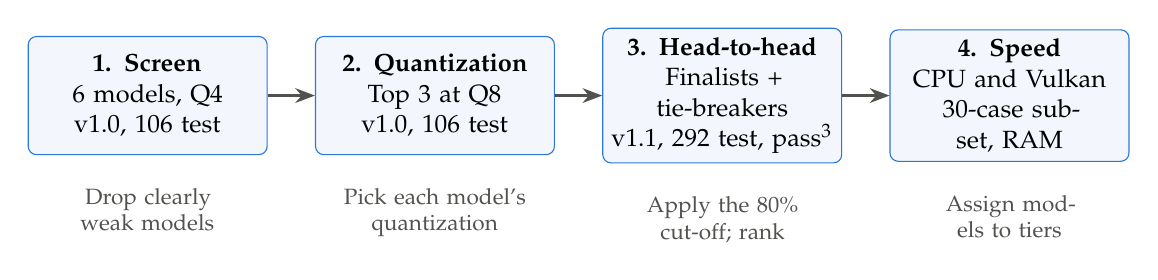
\begin{tikzpicture}[
  node distance=5mm and 6mm,
  stage/.style={draw=qblue, fill=boxfill, rounded corners=3pt, align=center, font=\small, minimum height=15mm,
                text width=28mm},
  arr/.style={-{Stealth[length=2.5mm]}, thick, ink2}]
\node[stage] (s1) {\textbf{1. Screen}\\6 models, Q4\\v1.0, 106 test};
\node[stage, right=of s1] (s2) {\textbf{2. Quantization}\\Top 3 at Q8\\v1.0, 106 test};
\node[stage, right=of s2] (s3) {\textbf{3. Head-to-head}\\Finalists + tie-breakers\\v1.1, 292 test, pass$^3$};
\node[stage, right=of s3] (s4) {\textbf{4. Speed}\\CPU and Vulkan\\30-case subset, RAM};
\draw[arr] (s1) -- (s2);
\draw[arr] (s2) -- (s3);
\draw[arr] (s3) -- (s4);
\node[below=3mm of s1, font=\footnotesize, text width=28mm, align=center, ink2] {Drop clearly weak models};
\node[below=3mm of s2, font=\footnotesize, text width=28mm, align=center, ink2] {Pick each model's quantization};
\node[below=3mm of s3, font=\footnotesize, text width=28mm, align=center, ink2] {Apply the 80\% cut-off; rank};
\node[below=3mm of s4, font=\footnotesize, text width=28mm, align=center, ink2] {Assign models to tiers};
\end{tikzpicture}
\caption{Staged evaluation protocol. Each stage narrows the field. Stage~3 uses the larger v1.1 test split, where
differences of about 6--7 points become detectable.}
\label{fig:stages}
\end{figure}

\subsection{Decision rules fixed in advance}\label{sec:rules}
These rules were written down before Stage~1 ran:
\begin{enumerate}
  \item \textbf{Cut-off.} A model is fit for deployment only if it reaches at least 80\% tool-call accuracy on the
        Stage~3 test split. The cut-off is reported as met or not met; it is not moved after results are known.
  \item \textbf{Ties go to the cheaper option.} When two quantizations of a model are statistically tied, the smaller
        and faster one is kept.
  \item \textbf{BF16 rule.} BF16 is downloaded and tested only if a finalist of 2B parameters or fewer shows a clear
        Q8-over-Q4 gain. Published quantization studies report that 4-bit quantization costs small models
        disproportionately more tool-calling accuracy than larger ones.
  \item \textbf{Selection.} Within each tier's memory budget, choose the configuration with the best Stage~3 quality.
        Use grounding (not inventing products) and then speed to break statistical ties.
\end{enumerate}
Two tie-breaker runs were added to Stage~3 after Stage~2 results were seen (Section~\ref{sec:decisions}). They extend
the comparison and do not change any rule, and they are reported as post-hoc additions.

\subsection{Reply-quality rubric}\label{sec:rubricmethod}
Automatic checks cannot judge whether a recommendation is well chosen, concise or friendly. In the test split, 88
discovery, comparison and Hinglish cases carry a four-line rubric (for example, ``Recommends only watches returned by the
tools'' or ``Questions target missing information that matters''). Each line is scored 1--5 for the two finalists'
greedy replies.

\begin{itemize}
  \item \textbf{Blinding.} A script built an anonymised packet for each case: the conversation, the rubric, any product
        data supplied to the model, and the two replies with their tool calls and results. The replies were labelled
        X and Y in a random order per case, and model names were removed. The key was kept separately.
  \item \textbf{Judge.} Scoring was done by a large general-purpose language model from a different model family than
        any candidate, which avoids the known tendency of a judge to favour its own family~\cite{llmjudge}. It ran as
        four independent instances, each scoring a quarter of the packet against written anchors (5 = fully meets the
        line; 1 = fails it). The instances had no access to the key.
  \item \textbf{Human check.} One evaluator scored 20 randomly drawn replies (about 10\%) on the same anchors, without
        seeing the judge's scores, to measure agreement.
\end{itemize}

% ===========================================================================
\section{Results}\label{sec:results}
% ===========================================================================

\subsection{Pilot and prompt correction}\label{sec:pilot}
A 30-case pilot with Qwen3.5-4B checked the harness end to end. It ran with no errors, 81\% prompt-cache reuse, and no
hidden thinking output. It passed 87\% of cases. Three of the four failures had the same cause: the system prompt told
the model to ask about budget and recipient before searching, while the evaluation labels expected an immediate search
whenever a specific feature was named. The prompt was rewritten to state the search-or-ask rule explicitly
(Appendix~\ref{app:prompt}). This was fixed before Stage~1, so every model was evaluated with the same corrected
prompt.

\subsection{Stage 1: screening}\label{sec:stage1}
All six models ran the v1.0 core set at Q4\_K\_M on Vulkan with no harness errors. Figure~\ref{fig:screen} shows the
test-split results.

\begin{figure}[H]
\centering
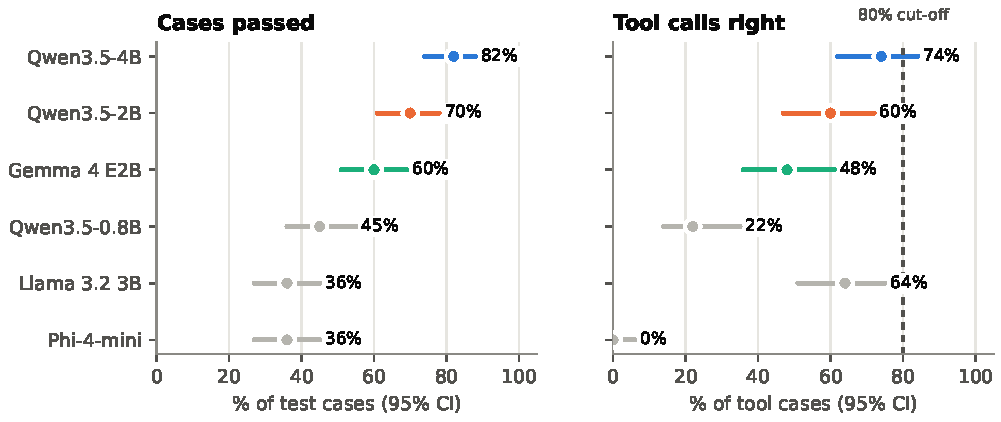
\includegraphics[width=\textwidth]{figs/fig_screen.pdf}
\caption{Stage 1 screen (Q4\_K\_M, 106 test cases). Left: cases passed. Right: tool-call accuracy on the 58 tool cases,
with the 80\% cut-off. Coloured models advanced to Stage~2. Whiskers are 95\% Wilson intervals.}
\label{fig:screen}
\end{figure}

\begin{itemize}
  \item \textbf{Qwen3.5-4B led} with 82\% [74--88]. It was significantly better than every other model in paired tests.
  \item \textbf{Qwen3.5-2B (70\%) and Gemma 4 E2B (60\%) came next}; the difference between them was borderline
        (9.4 points, interval [0.9, 17.9], $p = 0.053$).
  \item \textbf{The other three were well behind}:
  \begin{itemize}
    \item Qwen3.5-0.8B: 45\%;
    \item Llama 3.2 3B: 36\%;
    \item Phi-4-mini: 36\%.
  \end{itemize}
\end{itemize}

The two weakest models were read case by case, to establish whether they failed on ability or on format:
\begin{itemize}
  \item \textbf{Phi-4-mini made no structured tool calls in any case} (0\% tool-call accuracy). It asked for details or
        said it lacked access instead. In one case it wrote a tool call as plain text with an invented tool name. This
        is largely a format failure: llama.cpp's default template does not present tools in the format Phi-4-mini was
        trained on. There were real ability problems too. Without tool data, it invented specifications and dollar
        prices, claimed the store sold a brand it does not carry, and answered Hinglish in Devanagari script. Its
        grounded-answering pass rate (76\%) matched the leaders, which confirms the tool path as the main problem.
  \item \textbf{Llama 3.2 3B called tools correctly but could not stop.} In 73 of 150 cases it hit the four-round limit
        without replying, repeating calls with invented store IDs. It called tools on every no-tool question
        (0\% no-tool accuracy) and often sent numbers and lists as text strings. This is mostly an ability problem.
\end{itemize}
\textbf{Decision}: the top three advanced (Qwen3.5-4B, Qwen3.5-2B and Gemma 4 E2B).

\subsection{Stage 2: quantization}\label{sec:stage2}

\begin{figure}[H]
\centering
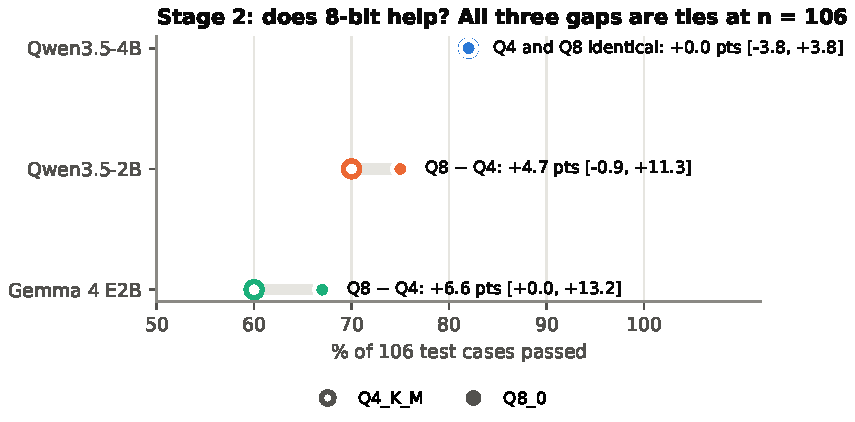
\includegraphics[width=0.78\textwidth]{figs/fig_quant.pdf}
\caption{Stage 2: Q4\_K\_M versus Q8\_0 on the same 106 test cases. Brackets give the paired-bootstrap 95\% interval
of the difference.}
\label{fig:quant}
\end{figure}

\begin{itemize}
  \item \textbf{Qwen3.5-4B}: Q8 scored exactly the same as Q4 (82\%, interval $\pm$3.8 points) while running about
        40\% slower. Q4 is kept.
  \item \textbf{The smaller models gained at Q8}, though neither gain was statistically clear at this sample size:
  \begin{itemize}
    \item Qwen3.5-2B: $+4.7$ points, interval [$-0.9$, $+11.3$];
    \item Gemma: $+6.6$ points, interval [0.0, $+13.2$].
  \end{itemize}
\end{itemize}
These gains were concentrated where small models are weakest. Qwen3.5-2B at Q8 improved on:
\begin{itemize}
  \item tool calls: 60\% $\to$ 69\%;
  \item Hinglish: 45\% $\to$ 73\%;
  \item naming real products: 73\% $\to$ 92\%.
\end{itemize}
The pattern (no gain at 4B, gains at 2B) matches the published finding that small models lose more to 4-bit
quantization. Because the gains were not significant, Stage~3 settles each small model's quantization with a
tie-breaker run on the larger set.

\subsection{Stage 3: head-to-head}\label{sec:stage3}
Stage 3 ran the v1.1 test split (292 cases, 168 needing a tool) for:
\begin{itemize}
  \item \textbf{Qwen3.5-4B Q4\_K\_M}: greedy, plus three runs at temperature 0.3;
  \item \textbf{Qwen3.5-2B Q4\_K\_M}: greedy, plus three runs at temperature 0.3;
  \item \textbf{tie-breakers, greedy only}:
  \begin{itemize}
    \item Qwen3.5-2B Q8\_0 (Q4 or Q8 for the 2B);
    \item Gemma 4 E2B Q8\_0 (2B or Gemma for the smaller slot);
    \item Qwen3.5-2B BF16, triggered by the BF16 rule (Section~\ref{sec:bf16}).
  \end{itemize}
\end{itemize}

\begin{figure}[H]
\centering
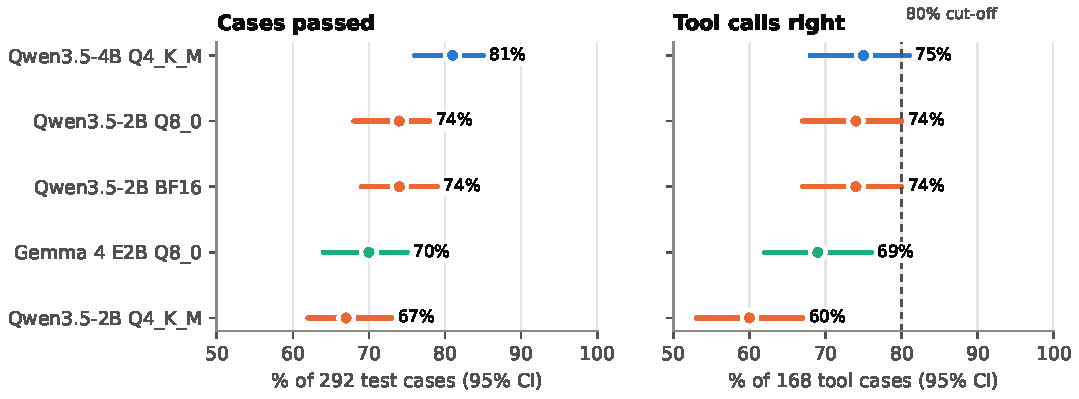
\includegraphics[width=\textwidth]{figs/fig_h2h.pdf}
\caption{Stage 3 (eval v1.1 test split, greedy decoding). Left: cases passed. Right: tool-call accuracy against the
80\% cut-off. No configuration reaches the cut-off.}
\label{fig:h2h}
\end{figure}

\begin{table}[H]
\centering
\small
\begin{tabular}{l r r r l}
\toprule
Comparison (same 292 cases) & Difference & 95\% interval & McNemar $p$ & Verdict \\
\midrule
Qwen3.5-4B Q4 vs Qwen3.5-2B Q8 & $+7.5$ & [$+2.4$, $+12.7$] & 0.007 & 4B better \\
Qwen3.5-2B Q8 vs Qwen3.5-2B Q4 & $+6.2$ & [$+1.4$, $+11.0$] & 0.015 & Q8 better \\
Qwen3.5-2B Q8 vs Gemma 4 E2B Q8 & $+4.1$ & [$-1.4$, $+9.9$] & 0.19 & Tie \\
Qwen3.5-2B BF16 vs Qwen3.5-2B Q8 & $+0.7$ & [$-2.1$, $+3.4$] & 0.80 & Tie \\
Qwen3.5-4B greedy vs temperature 0.3 & $+2.4$ & [0.0, $+5.1$] & 0.12 & Tie \\
\bottomrule
\end{tabular}
\caption{Key paired comparisons in Stage 3 (pass rate, percentage points).}
\label{tab:pairs}
\end{table}

\paragraph{Ranking.}
\begin{itemize}
  \item Qwen3.5-4B Q4 passed \textbf{81\%} [76--85] and was significantly better than every other configuration.
  \item Qwen3.5-2B Q8 passed 74\%, statistically ahead of its Q4 version (67\%) and tied with Gemma 4 E2B Q8 (70\%).
\end{itemize}

\paragraph{Reliability.} At temperature 0.3, Qwen3.5-4B averaged 79\% per run and had a pass$^3$ of 78\% [73--82].
Nearly every case it passes once, it passes every time. Qwen3.5-2B Q4 averaged 69\% with a pass$^3$ of 69\%.

\paragraph{The cut-off.} Tool-call accuracy was:
\begin{itemize}
  \item Qwen3.5-4B: \textbf{75\%} [68--81];
  \item Qwen3.5-2B Q8: \textbf{74\%} [67--80].
\end{itemize}
\textbf{Neither meets the 80\% cut-off}, and no other configuration came closer. Under the rules set in advance, this
is reported as not met.

\begin{figure}[H]
\centering
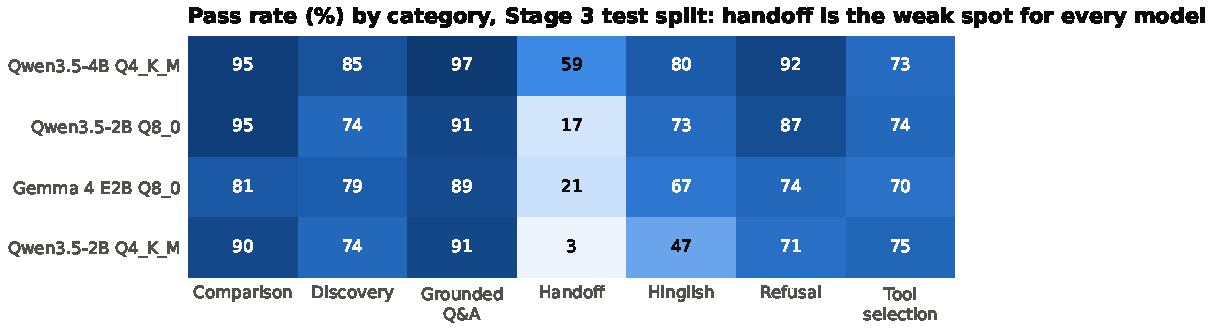
\includegraphics[width=\textwidth]{figs/fig_heat.pdf}
\caption{Stage 3 pass rate by category. Handoff (calling staff) is the weakest behaviour for every model; it is the
4B's largest advantage.}
\label{fig:heat}
\end{figure}

\paragraph{By category} (Figure~\ref{fig:heat}).
\begin{itemize}
  \item Comparison and grounded question answering are strong for every model (81--97\%).
  \item The models separate on:
  \begin{itemize}
    \item handoff: 59\% for the 4B against 3--21\% for the rest;
    \item Hinglish: 80\% against 47--73\%;
    \item refusals: 92\% against 71--87\%.
  \end{itemize}
\end{itemize}

\subsection{BF16 check}\label{sec:bf16}
Qwen3.5-2B's Q8-over-Q4 gain on 292 cases ($+6.2$ points, significant) met the BF16 rule, so Qwen3.5-2B was also run in
BF16. BF16 matched Q8 (74\%, difference $+0.7$, interval [$-2.1$, $+3.4$]) but was much more expensive on Vulkan:
\begin{itemize}
  \item generation speed: 8.3 tokens/s, against 13.9;
  \item peak memory: 5.8\,GB, against 3.6\,GB.
\end{itemize}
Q8\_0 is kept. Precision beyond 8 bits buys nothing for this task.

\subsection{Stage 4: speed and memory}\label{sec:stage4}

\begin{table}[H]
\centering
\small
\begin{tabular}{l l r r r r r}
\toprule
Configuration & Backend & Median s & p90 s & 1st token s & Tokens/s & RAM GB \\
\midrule
Qwen3.5-4B Q4\_K\_M & CPU & 15.5 & 51.0 & 1.42 & 9.2 & \textbf{6.1} \\
Qwen3.5-4B Q4\_K\_M & Vulkan & 12.1 & 34.4 & 1.85 & 9.8 & 5.7 \\
Qwen3.5-2B Q8\_0 & CPU & 11.5 & 29.7 & 0.70 & 15.0 & 2.7 \\
Qwen3.5-2B Q8\_0 & Vulkan & 7.4 & 17.0 & 0.72 & 13.9 & 3.6 \\
Qwen3.5-2B BF16 & Vulkan & 10.9 & 28.8 & 0.73 & 8.3 & 5.8 \\
Gemma 4 E2B Q8\_0 & CPU & 9.9 & 33.7 & 0.70 & 11.8 & 2.9 \\
Gemma 4 E2B Q8\_0 & Vulkan & 6.3 & 24.2 & 0.83 & 11.1 & 5.7 \\
\bottomrule
\end{tabular}
\caption{Stage 4 speed and memory on the fixed 30-case subset. Times are end to end per case, including all tool
rounds. Peak RAM is the inference server's resident memory.}
\label{tab:speed}
\end{table}

\begin{figure}[H]
\centering
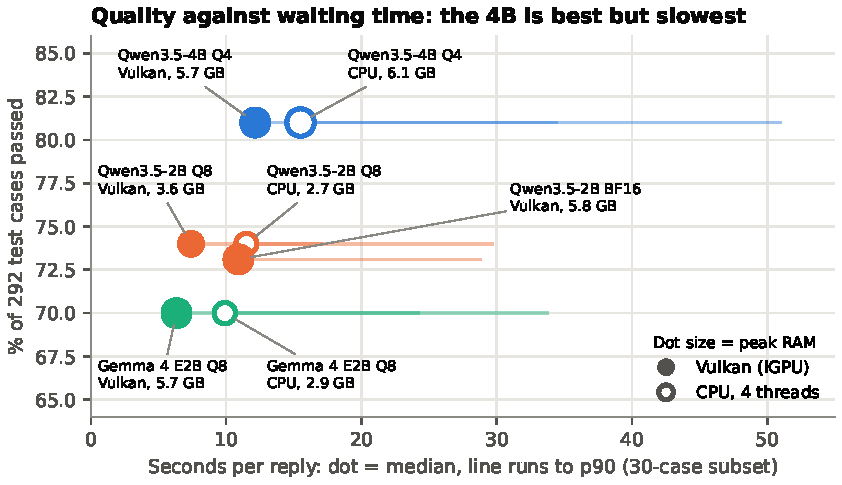
\includegraphics[width=0.86\textwidth]{figs/fig_tradeoff.pdf}
\caption{Quality (Stage 3 pass rate) against waiting time (Stage 4). Dots mark the median time per case, and lines extend
to the 90th percentile. Filled dots are Vulkan, hollow dots CPU, and dot area grows with peak RAM.}
\label{fig:tradeoff}
\end{figure}

Four observations follow from Table~\ref{tab:speed} and Figure~\ref{fig:tradeoff}:
\begin{enumerate}
  \item \textbf{The integrated GPU barely speeds up generation.} Tokens per second are about the same on CPU and Vulkan
        for every model, because the Iris Xe shares system memory and generation is limited by memory bandwidth.
        Vulkan's 20--40\% shorter replies come from faster prompt processing.
  \item \textbf{Qwen3.5-4B does not fit Tier~A.} It peaked at 6.1\,GB on CPU, above the 5\,GB budget, measured at an
        8K context. Both Qwen3.5-2B Q8 (2.7\,GB) and Gemma Q8 (2.9\,GB) fit.
  \item \textbf{Per-case times are not directly comparable across models}, because models make different numbers of
        tool calls: on this subset, 0.70 calls per case for Qwen3.5-2B, 0.47 for the 4B and 0.37 for Gemma. Each call
        adds a full round trip. Tokens per second is the fair speed comparison, and on it Qwen3.5-2B Q8 is fastest.
  \item \textbf{Tail latency is a usability risk.} 90th-percentile times of 17--51 seconds are long for a customer
        standing at a kiosk. The first token arrives in under 2 seconds, so streaming the reply would hide much of
        the wait.
\end{enumerate}
An early Stage~1 memory reading of 8.2\,GB for Qwen3.5-4B was not reproduced (5.7\,GB here). Resident-memory figures for
memory-mapped model files on Windows depend on how much of the file has been paged in, so all RAM figures should be
read as approximate.

\subsection{Failure analysis: why tool calls miss}\label{sec:failures}
All 168 tool cases were classified for the three strongest configurations (Figure~\ref{fig:failures}).

\begin{figure}[H]
\centering
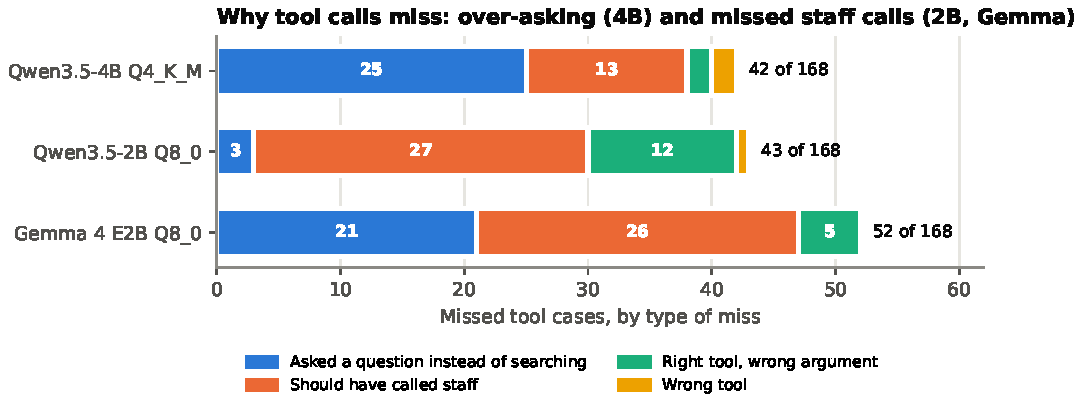
\includegraphics[width=0.92\textwidth]{figs/fig_failures.pdf}
\caption{Tool-call misses by type, Stage 3 test split.}
\label{fig:failures}
\end{figure}

Two behaviours account for about 90\% of misses:
\begin{itemize}
  \item \textbf{Over-asking (Qwen3.5-4B: 25 of 42 misses).} When the customer named a feature (``Show me chronographs'',
        ``Do you have titanium watches?'', ``Red dial watches?''), the 4B asked for budget and gender instead of
        searching. It did this in 17 of 21 feature-search cases, against an explicit prompt rule. The flip side: it
        asked correctly in 100\% of the cases where asking was right. It leans towards asking.
  \item \textbf{Missed handoff (Qwen3.5-2B: 27 misses; Gemma: 26).} For service requests (a battery change, cracked
        glass, a bracelet adjustment), the models asked which watch it was instead of calling staff. For unanswerable
        questions (engraving, shipping abroad, bulk discounts), they said they could not help and stopped. Across the three models, fifteen
        replies said a staff member would help without calling the tool. Most seriously, the 4B sometimes invented
        store policy instead of handing off (``Yes, we accept foreign credit cards''). These are scored as failures,
        and they are the clearest argument for a strict call-staff fallback.
\end{itemize}

One tool-design weakness also contributed. \texttt{search\_catalogue} has no field for case material, glass or
functions, and the free-text \texttt{query} field is described as being for ``a collection name or colour''. Qwen3.5-2B
therefore pushed features such as ``titanium'' or ``sapphire'' into unrelated filters (for example, style ``sport'' and
movement ``automatic''). When Gemma put ``titanium'' in \texttt{query}, the search worked.

\paragraph{Audit of the evaluation set.} Because both Qwen finalists sat at 74--75\% tool-call accuracy, the shared
failures were audited for labelling errors. No label error that changes a score was found. Two cases were too lenient
(they accepted a stock check for a ``similar watches'' request), and the mock search matched the generic word
``watch'', which makes keyword searches noisier. Both are logged for the next version. Stage~3 scores are reported
unchanged.

\subsection{Reply quality}\label{sec:rubric}

\begin{figure}[H]
\centering
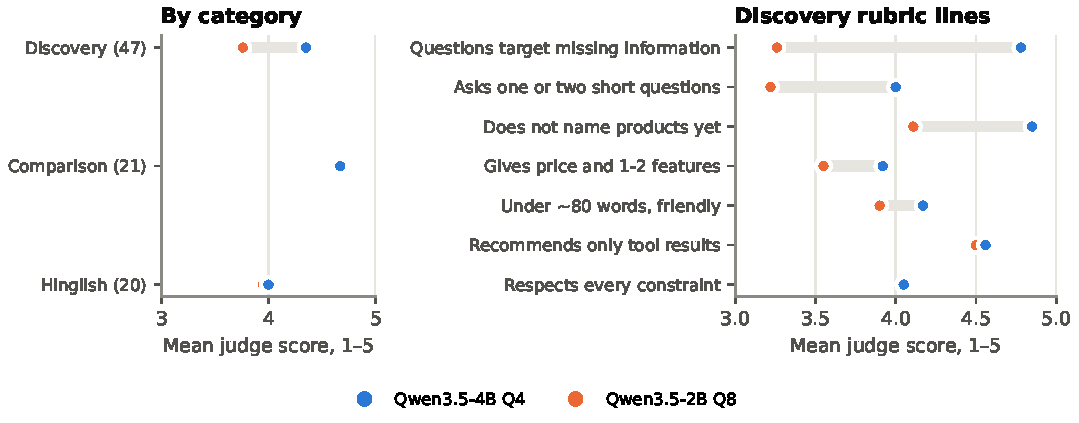
\includegraphics[width=\textwidth]{figs/fig_rubric.pdf}
\caption{Blind rubric scores (1--5) for the two finalists. Left: mean per category. Right: discovery rubric lines,
where the gap is concentrated.}
\label{fig:rubric}
\end{figure}

Over the 88 rubric cases:
\begin{itemize}
  \item \textbf{Mean case score:} Qwen3.5-4B 4.35, Qwen3.5-2B Q8 4.03.
  \item \textbf{Difference:} $+0.32$, interval [$+0.05$, $+0.59$], Wilcoxon $p = 0.045$.
  \item \textbf{Per case:} the 4B scored higher on 44, lower on 22, and tied on 22.
\end{itemize}

The gap comes almost entirely from \textbf{discovery} (4.35 against 3.76). When a question should come first, the 2B's
questions were less useful (3.26 against 4.78), and it named products too early. It also gave fewer prices and features
per watch. On comparison (4.67 against 4.71) and Hinglish (4.00 against 3.95) the two were equal. Both stayed
grounded: 4.56 and 4.50 on ``recommends only watches returned by the tools''.

\paragraph{Judge validity.}
\begin{itemize}
  \item \textbf{Agreement with the automatic check:} the judge's grounding scores averaged 5.0 where the automatic
        grounding check passed and 2.3 where it failed.
  \item \textbf{Agreement with the human evaluator:} on 70 rubric lines, 61\% exact agreement and 80\% within one
        point, with a quadratic-weighted $\kappa$ of 0.59 (moderate agreement).
  \item \textbf{The judge is stricter} than the human by 0.63 points on average, mainly on ``asks one or two
        questions'', where it penalised three or four questions as the rubric states, and on constraint lines.
\end{itemize}
Absolute rubric scores are therefore conservative. Both models were scored by the same judge, so the comparison between
them stands.

During this check, a defect in the blind packet was found and fixed. Ten comparison cases answer from supplied product
data, and that data had been left out of the packet, so the judge could not check those replies against it. The data was
added, and those ten cases were re-scored by a fresh judge instance under the same blinding. One human-check reply
affected by the defect was excluded from the agreement figures.

% ===========================================================================
\section{Decisions and reasoning}\label{sec:decisions}
% ===========================================================================

Table~\ref{tab:decisions} records every decision that shaped the result, the evidence behind it, and the reasoning.

{\small
\begin{xltabular}{\textwidth}{>{\raggedright\arraybackslash}p{3.3cm} >{\raggedright\arraybackslash}p{4.1cm} L}
\caption{Decision log.}\label{tab:decisions}\\
\toprule
Decision & Evidence & Reasoning \\
\midrule
\endfirsthead
\toprule
Decision & Evidence & Reasoning \\
\midrule
\endhead

Report two hardware tiers & Target kiosk hardware unknown & Lets the deployer pick from measured results instead of a guess.
Tier~A is a CPU-only box; Tier~B adds an integrated GPU. \\
Use a fictional catalogue & Retailer terms bar copying; internal data not public & A synthetic, seeded catalogue is
legal, reproducible, and lets internal fields and data defects be planted and tested on purpose. \\
Fix the prompt before Stage~1 & Pilot: 3 of 4 failures came from a prompt that contradicted the labels & A prompt that
contradicts the test measures the prompt, not the model. Fixing it before any candidate ran keeps the comparison
fair. \\
Staged protocol instead of a full grid & Full grid $>$50\,h; the backend changes speed, not answers & Quality is measured
once per model and quantization, and speed on a small subset. Weak models are dropped early on the smaller set. \\
Drop Phi-4-mini and Llama 3.2 3B & Stage~1: 36\% each; Phi made no structured calls; Llama looped & Both trailed the
third-placed model by 24.5 points (significant). Phi's failure is partly the default template; it is reported as
such, not as a verdict on the model. \\
Keep Qwen3.5-4B at Q4 & Q8 $-$ Q4 $= 0.0$ [$-3.8$, $+3.8$]; Q8 about 40\% slower & Tie, so the cheaper option wins
(rule 2). \\
Add tie-breaker runs to Stage~3 & Q8 gains of $+4.7$ and $+6.6$ points for the small models, not significant at $n = 106$ &
The smaller set could not settle these questions; the 292-case set can. Disclosed as post-hoc additions. \\
Qwen3.5-2B at Q8, not Q4 & $+6.2$ [$+1.4$, $+11.0$], $p = 0.015$ on 292 cases & A clear gain, and Q8 still fits Tier~A
(2.7\,GB on CPU). \\
Test BF16 for Qwen3.5-2B; keep Q8 & BF16 $-$ Q8 $= +0.7$ (tie); half the speed; 5.8\,GB & Required by rule 3 once Q8
beat Q4. BF16 adds cost without benefit. \\
Qwen3.5-2B over Gemma 4 E2B for Tier~A & Pass rate tied ($+4.1$, CI includes 0); names a real product 90\% vs 56\%;
faster generation & Statistically tied on overall quality, so grounding breaks the tie (rule 4): for a kiosk, not
inventing products matters most. Sharing the 4B's family also means one prompt and one template for both tiers. \\
\textbf{Tier B: Qwen3.5-4B Q4\_K\_M} & 81\% pass, best in every paired test; best handoff, Hinglish and refusal; rubric
$+0.32$ & Best quality within the 10\,GB budget (5.7\,GB). \\
\textbf{Tier A: Qwen3.5-2B Q8\_0} & 74\% pass; 2.7\,GB; 15 tokens/s on CPU & The 4B exceeds the 5\,GB budget on CPU.
The 2B is the best configuration that fits. \\
Do not move the 80\% cut-off & Tool-call accuracy 75\% and 74\% & The cut-off was set in advance. Moving it after
seeing results would defeat its purpose. It is reported as not met, and improvement is moved to Objective~2. \\
Use a blind, different-family judge with a human check & 704 rubric judgements; manual scoring impractical & Blinding and a
different model family limit bias. The human sample measures agreement; the result is stated with its caveats. \\
\bottomrule
\end{xltabular}
}

\paragraph{Selected models.}
\begin{itemize}
  \item \textbf{Tier B (integrated GPU, $\le$10\,GB): Qwen3.5-4B Q4\_K\_M.}
  \begin{itemize}
    \item 81\% of test cases passed; 75\% tool-call accuracy;
    \item 12.1\,s median reply; 5.7\,GB peak memory.
  \end{itemize}
  \item \textbf{Tier A (CPU only, $\le$5\,GB): Qwen3.5-2B Q8\_0.}
  \begin{itemize}
    \item 74\% of test cases passed; 74\% tool-call accuracy;
    \item 11.5\,s median reply; 2.7\,GB peak memory.
  \end{itemize}
\end{itemize}
Both selections carry the same qualification: \emph{neither reaches the 80\% tool-call cut-off}, so neither is fit for
unsupervised deployment as tested.

% ===========================================================================
\section{Limitations and threats to validity}\label{sec:limits}
% ===========================================================================
\begin{itemize}
  \item \textbf{Synthetic data.} The catalogue, policies and questions are generated. Real customer phrasing and real
        catalogue messiness may differ, and results should be re-checked on real data when it is available.
  \item \textbf{One machine.} Speed and memory were measured on one laptop that stands in for both tiers. Real kiosk
        hardware (including NPUs) may rank configurations differently on speed, though not on quality.
  \item \textbf{Single-turn harness.} Most cases are one customer turn. Behaviours such as asking which watch needs
        service before calling staff might be acceptable in a longer conversation, but are scored as misses here.
  \item \textbf{Default chat templates.} Every model used its own template as shipped in its GGUF file. Phi-4-mini in
        particular might perform differently with a template matched to its tool-call format.
  \item \textbf{Prompt sensitivity.} One prompt was used for all models. A prompt tuned for one model could change the
        ranking. Prompt work is deliberately left to Objective~2 and will be tuned on the dev split only.
  \item \textbf{Memory at 8K context.} RAM was measured at an 8,192-token context. Qwen3.5-4B might fit Tier~A at the
        4K context originally planned for that tier. This has not been tested.
  \item \textbf{LLM judge.} The rubric judge is stricter than the human evaluator, and agreement is moderate
        ($\kappa = 0.59$). Rubric results support the main ranking but are not used to make it.
  \item \textbf{Test-split reuse.} The Stage~3 test split has now been examined in detail. Any later improvement must
        be confirmed on freshly generated test cases, not on the same 292.
\end{itemize}

% ===========================================================================
\section{Next steps (Objective 2)}\label{sec:next}
% ===========================================================================
\begin{enumerate}
  \item \textbf{Prompt v1.2}: short examples of ``a feature is named, so search now'', and a hard rule that offering
        staff help means calling \texttt{call\_staff}. Tune on the 78 dev cases only.
  \item \textbf{Tool schema}: widen the \texttt{query} description to cover materials, glass and functions. Fix the
        search's match on generic words and the two lenient labels.
  \item \textbf{Fresh test set}: regenerate the expansion with a new seed for one confirming run of the final
        configuration against the 80\% cut-off.
  \item \textbf{Latency}: stream replies and shorten product lists to cut the perceived wait.
  \item \textbf{Scale}: regenerate the catalogue at 1,000--2,000 SKUs, where retrieval difficulty begins to matter.
\end{enumerate}

% ===========================================================================
\begin{thebibliography}{9}
\bibitem{llamacpp} G.~Gerganov and contributors. \emph{llama.cpp: LLM inference in C/C++}. Open-source software,
  \url{https://github.com/ggml-org/llama.cpp}.
\bibitem{bfcl} S.~G.~Patil et al. The Berkeley Function Calling Leaderboard (BFCL): From tool use to agentic evaluation of
  large language models. \emph{ICML}, 2025.
\bibitem{taubench} S.~Yao, N.~Shinn, P.~Razavi, K.~Narasimhan. $\tau$-bench: A benchmark for tool-agent-user interaction
  in real-world domains. arXiv:2406.12045, 2024.
\bibitem{wilson} E.~B.~Wilson. Probable inference, the law of succession, and statistical inference. \emph{Journal of
  the American Statistical Association}, 22(158):209--212, 1927.
\bibitem{mcnemar} Q.~McNemar. Note on the sampling error of the difference between correlated proportions or
  percentages. \emph{Psychometrika}, 12(2):153--157, 1947.
\bibitem{efron} B.~Efron and R.~J.~Tibshirani. \emph{An Introduction to the Bootstrap}. Chapman \& Hall, 1993.
\bibitem{errorbars} E.~Miller. Adding error bars to evals: A statistical approach to language model evaluations.
  arXiv:2411.00640, 2024.
\bibitem{llmjudge} L.~Zheng et al. Judging LLM-as-a-judge with MT-Bench and Chatbot Arena. \emph{NeurIPS Datasets and
  Benchmarks}, 2023.
\end{thebibliography}

% ===========================================================================
\appendix
\section{Tool-mode system prompt}\label{app:prompt}
\begin{small}
\begin{verbatim}
You are the shopping assistant on an in-store kiosk at a Veyra watch store.
Help customers find, compare and check watches.
Rules:
- Use the tools for product details, prices, stock and alternatives. Never
  invent product IDs, prices, specs or stock.
- Search right away when the customer gives a product ID, names any specific
  feature (material, glass, strap type, dial colour, collection or sub-brand,
  movement, functions such as chronograph or luminous hands, digital or
  analog, water resistance, case size), or gives both a budget and who the
  watch is for.
- If the request is too general to search (only a budget, only who it is
  for, only an occasion, or only a general style such as 'sporty' or 'big'),
  ask one or two short questions first.
- If the information is not in the tool results or the store information,
  say so plainly. Do not guess.
- Call staff when the customer wants to try on or buy a watch, needs a repair
  or service, asks for a manager, or asks something you cannot answer.
- Never reveal internal information such as cost prices, margins or staff
  notes. Do not offer discounts beyond the current offers.
- Reply in the customer's language (English, Hindi or Hinglish). Keep replies
  under 80 words.
\end{verbatim}
\end{small}

\section{Run configuration}\label{app:config}
\begin{small}
\begin{tabularx}{\textwidth}{l L}
\toprule
Setting & Value \\
\midrule
Inference server & llama.cpp \texttt{llama-server}, one fixed build for all runs \\
Server flags (Vulkan) & \texttt{--jinja -c 8192 -np 1 -ngl 99} \\
Server flags (CPU) & \texttt{--jinja -c 8192 -np 1 -ngl 0 -t 4} \\
Qwen3.5 thinking & Off: \texttt{--reasoning-budget 0} and \texttt{enable\_thinking: false} per request \\
Decoding & Temperature 0, seed 42, at most 512 tokens per turn; reliability runs at temperature 0.3, 3 repeats \\
Tool loop & Up to 4 model--tool rounds per case \\
Prompt caching & Enabled; about 80\% of prompt tokens reused \\
Memory measurement & Peak resident set size of the server process, sampled by a separate monitor \\
Hardware & Intel Core i5-1240P, 16\,GB RAM, Intel Iris Xe graphics, Windows~11 \\
\bottomrule
\end{tabularx}
\end{small}

\end{document}
